\section{Aufbau und Durchführung}
\subsection{Aufbau}
\label{sec:Aufbau}

Der Versuchsaufbau ist in Abbildung \ref{fig:aufbau1} dargestellt.
Der Aufbau ist ein Resultat aus einer Start-Stopp-Messmethode und zusätzlichen Elementen, um diverse Fehlerquellen zu reduzieren.\\

\begin{figure}
  \centering
  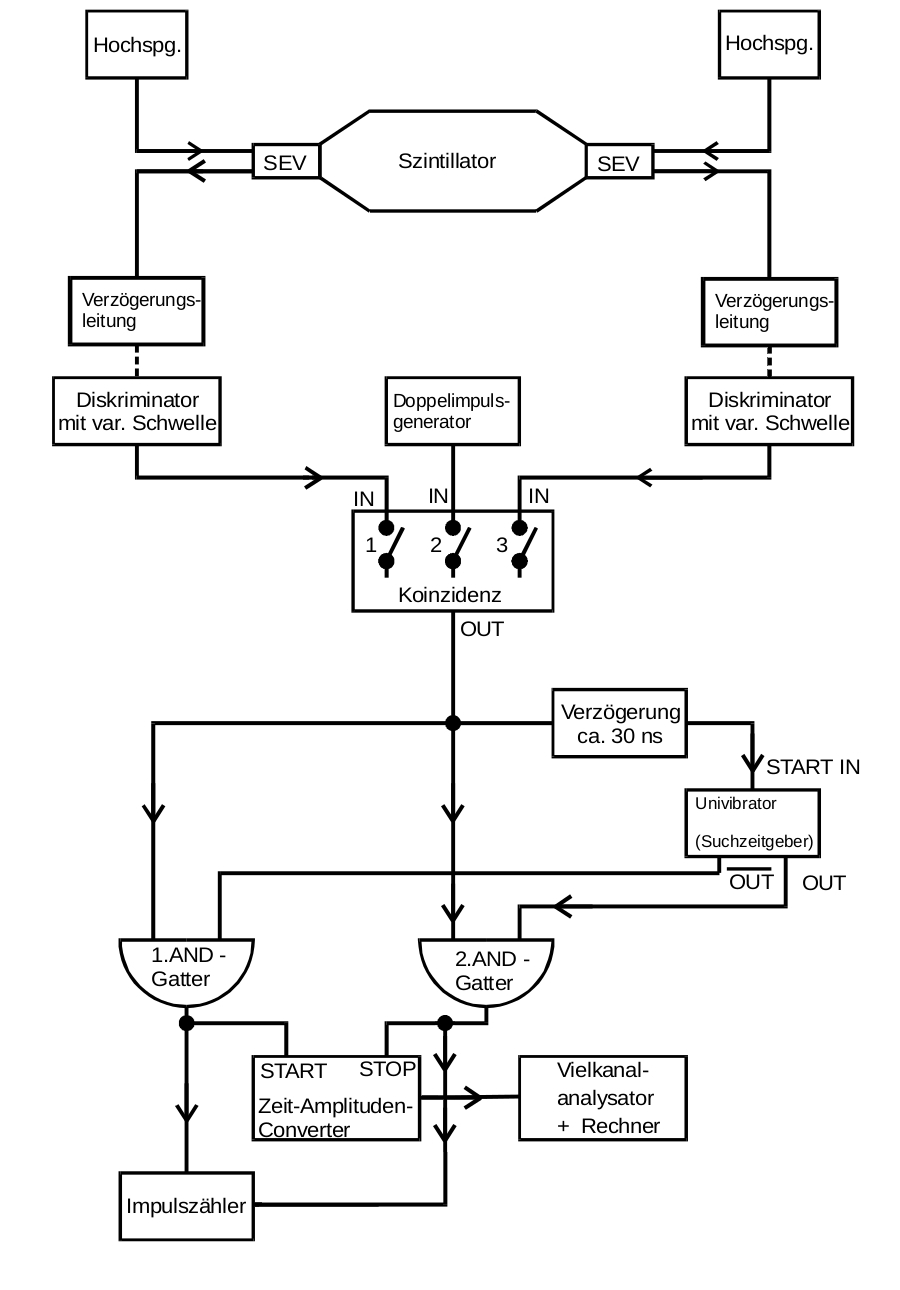
\includegraphics[height=15.5cm]{ressources/aufbau.jpeg}
  \caption{Systematischer Aufbau einer Apparatur, um die Lebensdauer von Myonen zu bestimmen \cite{skript}, modifiziert mit einer zusätzlichen Verzögerungsleitung am rechten SEV und Zählung der Stoppimpulse.}
  \label{fig:aufbau1}
\end{figure}



Die Apparatur besteht aus einem organischen Szintillationsdetektor.
Als Lösungsmittel wird Toluol verwendet, da die Abklingdauer dieses Materials mit etwa $\SI{10}{\nano\second}$ zwei Größenordnungen kleiner ist als die mittlere Lebensdauer eines Myons.
Wenn ein Myon in den Detektor eintritt, gibt es seine kinetische Energie an die Moleküle des Szintillatormaterials ab, welche dadurch in einen angeregten Zustand übergehen.
Bei der Rückkehr in den Grundzustand wird dementsprechend ein Lichtimpuls emittiert.
Zerfällt nun das Myon im Szintillator, entsteht ein Elektron, welches, wie zuvor das Myon, seine kinetische Energie an das Szintillatormaterial abgibt.
Es entsteht erneut ein Lichtimpuls.
Der Abstand der beiden Lichtimpulse ist dabei die Individuallebensdauer des Myons.
Die Lichtimpulse werden von Photokathoden in elektrische Signale umgewandelt.
Die daran anschließenden Sekundärelektronenvervielfacher (SEV) verstärken das elektrische Signal.
Da es bei endlicher Temperatur in dem SEV zu thermischer Emission von Elektronen kommen kann, werden zwei SEVs eingesetzt, welche eine Koinzidenz durchlaufen.
Weil diese thermische Emission der beiden SEVs unkorreliert sind, können diese Fehlimpulse durch die Koinzidenz herausgefiltert werden.
Hierbei wird eine Verzögerungsleitung eingesetzt, da die SEVs verschiedene elektronische Eigenschaften und Kabellängen besitzen.
Die Impulse ausgelöst durch die Myonen werden dabei nicht herausgefiltert, da der zeitliche Abstand eines Fehlimpulses an dem einen SEV und eines Fehlimpulses an dem anderen SEV in der Regel größer ist als der zeitliche Abstand der Impulse, ausgelöst durch ein Myon, welcher seinen Grund in der räumlichen Ausdehnung des Szintillators hat.\\
Die Diskriminatoren erfüllen mehrere Funktionen.
Zunächst wandeln sie das elektrische Signal, welches aus den SEVs kommt, in einen elektrischen Impuls mit fest definierter Breite und Höhe um, der von der Logik des NIM-Standards verarbeitet werden kann.
%Die Breite des Signals bestimmt, welche es durch die Koinzidenz schaffen.
Die Koinzidenz leitet die Signale nur weiter, wenn die beiden Signale der Diskriminatoren innerhalb einer gewissen Zeitspanne auftreten.
Ob ein Signal weitergegeben wird, hängt von den Breiten der einzelnen Signale und der Verzögerungsleitung vor den Diskriminatoren ab.
%Die Auflösungszeit hängt von der Verzögerungsleitung und der Breiten der Signale ab.
Die Zeitspanne, in der die Koinzidenz zwei Impulse als "gleichzeitig" identifiziert, sollte größer sein als $\SI{4}{\nano\second}$, dem Fall, in dem ein Lichtimpuls direkt an einer der Photokathoden ausgelöst wird.
Des Weiteren lassen die Diskriminatoren nur Impulse durch, welche eine festgelegte Spannungsschwelle überschreiten.
Da die Impulse, ausgelöst durch die thermische Emission in den SEVs, in der Regel viel kleiner sind als die, welche von Myonen ausgelöst werden, können somit diese Fehlimpulse zusätzlich herausgefiltert werden.\\
An einem Eingang der Koinzidenz befindet sich aus Justagezwecken ein Doppelimpulsgenerator, welcher ein $\SI{1}{\kilo\hertz}$-Signal in einem in $\SI{0,1}{\micro\second}$-Schritten einstellbaren Abstand aussendet.\\
Auf die Koinzidenz folgt die Logik, welche die Lebensdauer der Myonen misst.
Im Idealfall erzeugt das Myon, welches in den Tank fällt, einen Startimpuls.
Selbiges erzeugt beim Zerfall einen Stoppimpuls.
Der Startimpuls geht an den START-Eingang eines Zeit-Amplituden-Converters (TAC), sowie der Stoppimpuls an den STOP-Eingang.
Der TAC gibt einen Impuls aus, dessen Höhe proportional zum Zeitunterschied zwischen Start- und Stoppsignal ist.
Dieses Signal wird von einem Vielkanalanalysator je nach Höhe einem Kanal zugeordnet und zu einem Rechner weitergeleitet.
Das auf dem Rechner vorinstallierte Programm speichert die Anzahl der Impulse pro Kanal ab.\\
Das Aussehen der Schaltung resultiert jedoch daher, dass ein Großteil der Myonen den Tank durchquert, ohne zu zerfallen.
Daher gäbe es einen Start- aber keinen Stoppimpuls.
Um dies zu beheben wird eine monostabile Kippstufe eingesetzt, welche eine einstellbare Suchzeit $T_\text{S}$ besitzt.
Der Ausgang der Koinzidenz wird an die Eingänge zweier UND-Gatter und an den Eingang der monostabilen Kippstufe angeschlossen.
Der inverse Ausgang der Kippstufe wird an das UND-Gatter angeschlossen, dessen Ausgang mit dem START-Eingang des TAC verbunden ist.
Der nicht inverse Ausgang geht an das andere UND-Gatter, welches an den STOP-Eingang des TAC geht.
Damit ein Startimpuls den TAC startet, wird eine im Vergleich zur Lebensdauer des Myons sehr kleine Verzögerung vor die Kippstufe geschaltet, sodass das erste UND-Gatter das Startsignal weiterleiten kann.
Mit dem Startsignal wird die Suchzeit $T_\text{S}$ der Kippstufe gestartet.
Der TAC kann daher nur gestoppt werden, wenn während der Suchzeit ein zweites Signal auftaucht.
Ist dies nicht der Fall, wird mit dem nächsten Signal der TAC wieder gestartet.
Die Suchzeit sollte größer als die Lebensdauer eines Myons, aber auch sehr viel kleiner sein als der zeitliche Abstand, in dem ein anderes Myon in den Tank eintritt.
Im Durchführungskapitel wird darauf quantitativ näher eingegangen.
Es kann jedoch immer passieren, dass sich zwei Myonen im Tank befinden.
Dieser Untergrund ist hinreichend gleichmäßig über alle aufgenommenen Zeitintervalle verteilt und ist abhängig von der Suchzeit, der Messzeit und der Gesamtzahl der Startimpulse.
Daher wird zusätzlich an den Ausgang des ersten UND-Gatters ein Impulszähler zugeschaltet, welcher die Startimpulse zählt.
Zusätzlich werden die Stoppimpulse gezählt.
